\subsection{Test Doubles}
%Test doubles / isolation
%Moq framework +example
The way our code is written, we have a certain focus on the room, wherein the other actors may reside. This means that a lot of the methods requires a specified room, to know where and what to look for. In short, we have high coupling between our classes. However, in unit testing, we wish to perform tests of each class in isolation, independently of the other classes. So, if we have high coupling, and yet want to test classes independently, how are we to do this? \\ This is where test doubles come in. Using test doubles, also known as scaffolding, is the means of making it easier to isolate code for testing. The point of a test double is to act as a class, including some of its functionality, so that it can be used by another class that is being tested\cite{TestingCodeComplete}. There are various test doubles available, such as fakes, dummies and mocks. Since mocking is what we are going to use, this is what we will look more into.

\subsubsection{Mocking} \label{MockingSection}
The idea of mocking, or mock objects, is to mimic the behaviour of the real class we are imitating. However, we can do this in a controlled way, such that the methods of the mimicked class returns some specific values, independently of the input they receive. This means that the class will not produce any specific results based on their real implementation, but predefined output that we specify\cite{TestingAdaptiveCode}. As such, if we have a class we want to test, that is dependent on the class we mimic, we can now replace the dependency with our mimicked class. Now we have isolated the class we want to test, as all interactions with the mimic is controlled. \\
\\
To mimic the behaviour of a real class it would require us to make a new class. For each class we would like to mimic, we would have to make seperate classes for. This does not only mean that we would need a lot of extra code just for our unit tests, but also that if we were to change the actual class, we would have to change the mimic. This could, potentionally, become tedious work. To get around this, we make use of a framework, that enables us to make the mock objects dynamically, namely the Moq Framework.

\subsubsection{Moq Framework}
This will serve as a short introduction to the Moq framework and how we use it in our testing. \\
We already mentioned how making our mocked versions of the various classes manually would be tedious work. Luckily, the Moq framework makes it easy for us to mock a given class. This framework is very powerful as it allows us to manipulate the behaviour and expectations of our class\cite{TestingAdaptiveCode}. The major part of the mocking lies in the setup. When setting up a new mock, you can specify with the help of the Setup() function, what a given function should return, based on some specific or generic input. Let us take a closer look at the first line of the function body in \autoref{TakeTestMoq}. 
\begin{figure}
    \centering
    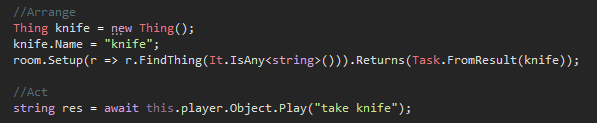
\includegraphics[width=0.9\linewidth]{Materials/TestingTheory/testTakeTestMoqExample}
    \caption{Part of player's TakeTest() showcasing the moq framework's setup}
    \label{TakeTestMoq}
\end{figure}
Here, we can see a nice example of the moq framework. The variable here, room, is of Mock<IRoomGrain>. As we can see with the lambda function, we specify that by a call to the room's FindThing() function, with an input of type string should return the newly created knife. This way, we can test the player's take command, that requires the room we are currently in, as well the items in this room, without the interaction of an actual room. This ensures that we can test the player in isolation, while also noting that the player indeed does send a message to the room grain. It should also be noted here, that while player is of type Mock<PlayerGrain>, by calling player.Object we effectively have the mocked player of type IPlayerGrain and not a player of type Mock<PlayerGrain>.

\subsubsection{Mocking a Class vs Mocking an Interface} \label{MockingVsSection}
We would also like to shortly explain the difference between mocking a class and mocking an interface. As is made apparent in our tests, we mock both the class under testing and the classes that it depends on. The only difference in the mocking between these two is that the class under testing is a mock of the actual class, while its dependencies are mocks of their interfaces. \\
Mocking an interface creates an instance of the class that implements this interface, but with no actual implementation or logic. For instance, if we look at \autoref{TakeTestMoq}, we set the room's FindThing() function to return a knife to us. If we did not do this setup, the function would not have been implemented and given us the default value of the given type instead. In the case of FindThing() it would have given us null. \\
Mocking a class creates an inherited class of the mocked one, which per standard uses the base implementation of their functions. So if we mock a class and make no setup, the functions will be the same. However, the smart thing about mocking these classes for testing, that function virtually the same as the original class, is that it allows us to change certain behaviour, while still maintaining the same functionality, such that we can test it properly. \\
We will look more into why this is important, and how we have changed certain aspects of the code, in the subsection '\nameref{GrainFactorySection}'. \todo{Siden det er subsec, nævn sec den er under?}

%Gem GrainFactory for discussion
% \begin{figure}
%     \centering
%     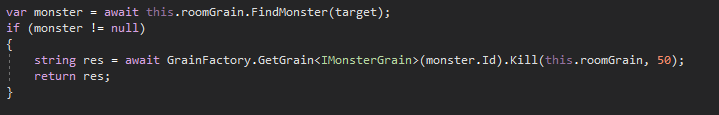
\includegraphics[width=\linewidth]{Materials/TestingTheory/FireballGrainFactory}
%     \caption{Snippet of player's Fireball() function, showcasing the problem with GrainFactory. Even if our room was mocked and returned our mocked monster's id, GrainFactory would create a real monster based on this id, as it finds no monsters with this id.}
%     \label{fireballGrainFactory}
% \end{figure}
% However, we do still have a problem, since this mocking does not cover all of our coupling of the grains. We can access different grains by calling GrainFactory.GetGrain<Type>(id), but by the nature of grains, if we call this function, with an id that does not correspond to any existing grain, it will automatically generate one for us. These methods are called inside some of the different functions of our grains, meaning that even though we can mock a monster, if a function inside player calls a function inside monster through the use of GrainFactory, it will ignore any mock monster we have created and make a real IMonsterGrain for us instead. We can see this problem illustrated in \autoref{fireballGrainFactory}. \todo{Måske cite + billede er godt til at illustrere?} So, how do we get around this? \\
% One way to side-step this issue is to mock the GrainFactory function of the class we are currently testing. To do this, we have to expose the GrainFactory function of the class, as it normally is a protected function. We would then create an override of the GrainFactory function, which means that we rewrite code in our classes due to our tests and while this is bad practice, it must be done in order to mock the GrainFactory and ensure that our grains do not make their own grains when we want them to use our mocked grains instead \todo{cite?}. \\ 
% This does open yet another issue. The new GrainFactory implementation cannot be part of our interface, such that if we want to use our mocked GrainFactory, we would use mocks of the classes instead of the interfaces (e.g. Mock<PlayerGrain> instead of Mock<IPlayerGrain>), rendering some of the interfaces functions hidden and unsuable for testing. \todo{Billeder? what to do med problemet? "maskintekst" for funktioner i vores tekst?}